\newpage
\hypertarget{t2m close}{}
\subsection{Tree To Model Close}
\genHeader

\begin{itemize}

\item[$\blacktriangleright$] Update TGG main from \texttt{box} to \texttt{tree}.

\item[$\blacktriangleright$] Navigate to ``src/org.moflon.tie'' right click and run as application

\item[$\blacktriangleright$] Will naturally have one error saying it wasn't able to complete the reverse transformation (we haven't built it yet; will do next)
but if you refresh your instances folder and open \texttt{tree.xmi\_fwd.xmi} you'll be able to see the model output (as a tree) of your original text/folder
file hierarchy.

\begin{figure}[htbp]
\begin{center}
  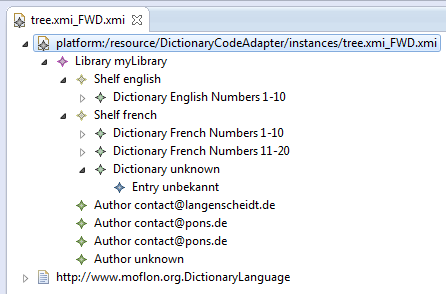
\includegraphics[width=0.7\textwidth]{ea_modelToTreeResult}
  \caption{completed NodeToDictionary}
  \label{ea:NodeToDictionary_Complete}
\end{center}
\end{figure}

\item[$\blacktriangleright$] If you haven't already, read Section 6 from Part IV to learn how eMoflon's integrator feature can help you visualize how this
transformation was completed. Note that this tool can also be useful for debugging if your TGG doesn't succeed.

\end{itemize}